\documentclass[12pt]{article}

\usepackage{mathtools}
\usepackage{amsfonts}
\usepackage{amsthm}
\usepackage{amssymb}
\usepackage{relsize}
\usepackage[margin=1in]{geometry}
\usepackage{graphicx}
\usepackage{dblfloatfix}
\usepackage[font=normalsize,labelfont=bf]{caption}
\usepackage{amsmath}
\usepackage{textcomp}
\usepackage{hyperref}
\usepackage{listing}
\usepackage{listings}
\usepackage{calc}
\usepackage{xcolor}
\usepackage{empheq}




\graphicspath{ {../data/} }

\newtheorem{theorem}{Theorem}[section]
\newtheorem{corollary}{Corollary}[theorem]
\newtheorem{lemma}[theorem]{Lemma}
\newtheorem{definition}{Definition}[section]

\newcommand{\ltwonorm}[1]{\|#1\|_2^2}
\newcommand{\tran}[1]{#1^T}

\definecolor{codegreen}{rgb}{0,0.6,0}
\definecolor{codegray}{rgb}{0.5,0.5,0.5}
\definecolor{codepurple}{rgb}{0.58,0,0.82}
\definecolor{backcolour}{rgb}{0.95,0.95,0.92}

\lstdefinestyle{mystyle}{
    backgroundcolor=\color{backcolour},
    commentstyle=\color{codegreen},
    keywordstyle=\color{magenta},
    numberstyle=\tiny\color{codegray},
    stringstyle=\color{codepurple},
    basicstyle=\ttfamily\footnotesize,
    breakatwhitespace=false,
    breaklines=true,
    captionpos=b,
    keepspaces=true,
    numbers=left,
    numbersep=5pt,
    showspaces=false,
    showstringspaces=false,
    showtabs=false,
    tabsize=2
}

\lstset{style=mystyle}

\title{Video Object Segmentation}
\author{Shir Hamawie \& Nadav Shoham}
\date{\today}

\begin{document}
\maketitle
    \section{Introduction}\label{sec:intro}
    Video object segmentation is a task in computer vision that involves extracting the foreground objects of interest from a video sequence.
    One way to perform this task is by a semi-supervised video object segmentation method.
    This method leverages only one manual annotation in the initial frame of the video, known as the ground-truth mask, and aims to propagate this annotation to subsequent frames in an unsupervised manner. \\
    In this assignment, we aim to design and implement that, based on Or Dinari's ScStream code as a building block.
    The ScStream code provides a foundation for processing video streams efficiently. \\
We will use two videos, one of a walking 3D dinosaur and another of a swimming swan as our test cases, each of them has it's own challenges and characteristics:
\begin{figure}[h!]
    \begin{minipage}{0.5\textwidth}
    \centering
    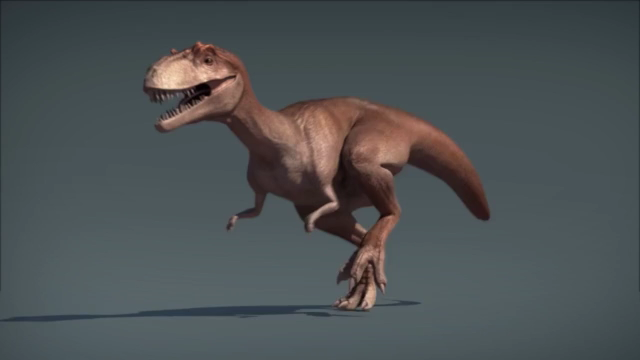
\includegraphics[scale=0.4]{images/dinosaur/first_frame_ratio1.0}
    \end{minipage}
    \begin{minipage}{0.5\textwidth}
    \centering
    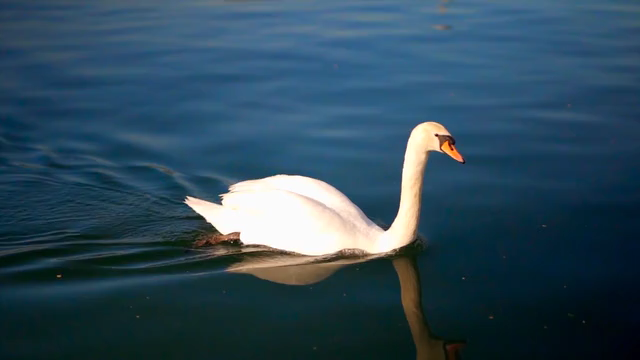
\includegraphics[scale=0.4]{images/swan/first_frame_ratio1.0}
    \end{minipage}
    \caption{First Frames}
    \label{fig:first_frames}
\end{figure}

The remainder of this report is organized as follows:
    \begin{itemize}
        \item \underline{Section 2 - } provides a brief overview of Or Dinari's ScStream.
        \item \underline{Section 3 - } we describe the methodology and architecture in detail.
        \item \underline{Section 4 - } presents the critical points that most influenced the application.
        \item \underline{Section 5 - } results and conclusion.
    \end{itemize}

\pagebreak
    \section{Background}\label{sec:background}
        \subsection{DP-Means}\label{subsec:dpmeans}
DP-Means is a clustering algorithm based on the Dirichlet Process Mixture Model (DPMM).
It aims to automatically determine the number of clusters in a dataset without requiring a predefined number of clusters.
However, DP-Means can be computationally expensive, especially for large datasets, as it involves calculating pairwise distances between data points.
        \subsection{PDC-DP-Mean}\label{subsec:pdc}
PDC-DP-Means is a method proposed by Or Dinari and Freifeld in 2022 that builds upon the DP-Means algorithm.
PDC-DP-Means is designed to address the limitations of traditional DP-Means in terms of scalability and computational efficiency.
PDC-DP-Means introduces parallelism and delayed cluster creation to improve the scalability and efficiency of DP-Means.
By leveraging parallel computing techniques, PDC-DP-Means can distribute the computational load across multiple threads or machines, enabling faster processing of large datasets.
This parallelization significantly reduces the runtime of the algorithm.
Additionally, PDC-DP-Means incorporates delayed cluster creation, which allows for more efficient memory usage.
Instead of creating clusters for all data points at once, PDC-DP-Means delays the creation of clusters until they are needed.
This approach reduces the memory requirements of the algorithm, making it more suitable for handling large-scale datasets.
The combination of parallelism and delayed cluster creation in PDC-DP-Means results in a highly scalable and efficient algorithm for clustering.
It enables the algorithm to handle large datasets with improved computational speed and reduced memory usage compared to traditional DP-Means.
        \subsection{ScStream}\label{subsec:scstream}
ScStream is a method proposed by Or Dinari and Freifeld in 2022 that builds upon the principles of DPMM.
It is specifically designed for clustering streaming data, where data arrives in a continuous and sequential manner.
ScStream leverages the sampling-based approach of DPMM to perform clustering on streaming data efficiently.
The key advantage of ScStream is its ability to handle any exponential family, making it suitable for a wide range of data types.
It offers a fast implementation that can work in either multi-threaded mode or multi-machine multi-process mode, enabling scalability and parallelization.
\pagebreak

\section{Methodology}\label{sec:methodology}
Our proposed method for semi-supervised video object segmentation consists of several key steps, which we will outline in detail.
The overall workflow follows a sequential process at each iteration, starting with foreground and background extraction,
followed by ScStream model training, and finally the creation of Gaussian data mixtures to be used in the next iteration.
The central method of our implementation is the \textbf{segment} method in \textcolor{red}{video\_object\_segmentation.py}.
\subsection{First Frame}\label{subsec:first-frame}
\subsubsection{Initial Foreground and Background Extraction}\label{subsubsec:initial-foreground-and-background-extraction}
The first step of our method involves extracting the foreground and background regions from the initial frame of the video.
To accomplish this, we employ the \textbf{GrabCut} algorithm, a popular technique for interactive foreground extraction in images.
The GrabCut algorithm combines color and spatial information to iteratively refine the foreground and background segmentation.
It requires an initial bounding box or a rough mask specifying the location of the foreground object.
In our case, this a great option to define the ground-truth mask of the object in the first video frame, since it is a semi-supervised method.
Our implementation of GrabCut uses the OpenCV library and can be found in the \textcolor{red}{grab\_cut.py} file.
Example result:
\begin{figure}[h!]
    \begin{minipage}{0.5\textwidth}
    \centering
    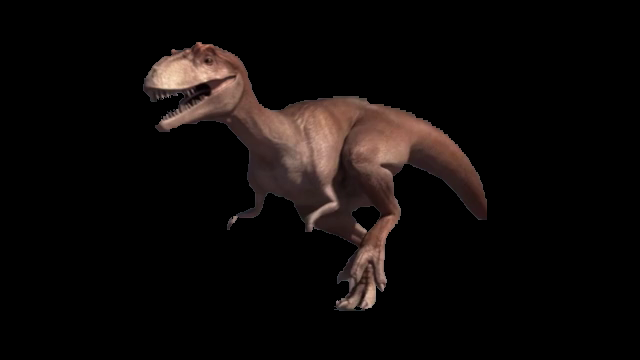
\includegraphics[scale=0.4]{images/dinosaur/foreground_ratio1.0}
    \caption{Foreground}
    \end{minipage}
    \begin{minipage}{0.5\textwidth}
    \centering
    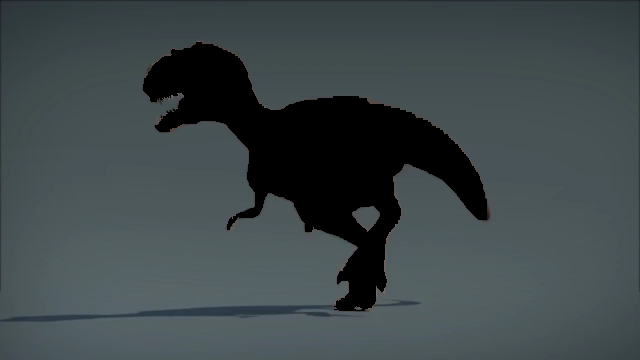
\includegraphics[scale=0.4]{images/dinosaur/background_ratio1.0}
    \caption{Background}
    \end{minipage}\label{fig:foreground extraction}
\end{figure}

\subsubsection{Models Initialization}
Once the foreground and background regions of the current frame have been extracted, we proceed to initialize our models.
Our goal is to be able to classify data to foreground and background by their characteristics.
Therefore, creating a model for each of them will create two separate and different gaussians that we can later extract from the models and use as our classifiers.
When initializing our models with \texttt{fit\_init} we have to do some hyper-parameter tuning that we will discuss in the next section.
Also, we want to let \texttt{fit\_init} run until convergence, since the initial run is on the ground-truth data and we want the model to learn it accurately.
\pagebreak
\subsection{Segmentation Loop}\label{subsec: segment-loop}
\subsubsection{Creation of Gaussian Data Mixtures}\label{subsubsec:gaussians}
As previously said the gaussians of the foreground and background models are our classifiers, helping us determine how to separate a new frame into 2 parts.
we can build them by extracting the means and covariances of the clusters from each model and initialize a \textbf{GaussianMixture} instance for both of them.
The GaussianMixture class is defined in \textcolor{red}{gaussian\_mixture.py} and uses \texttt{Scipy.stats.multivariate\_normal} to represent each gaussian.
The class supports two pdf options, pdf of the mixture using weights and sum of all gaussians pdfs, and max pdf that returns the gaussian pdf with the largest value.
\lstinputlisting[language=Python, firstline=7, lastline=20,label={lst:gaussians}]{../gaussian_mixture.py}
\subsubsection{Foreground and Background Extraction}\label{subsubsec: fg-bg-extract}
Now that we can no longer supervise the separation of the foreground and background we need to define a decision rule
that exploits the given gaussianMixtures and classifies each pixel in the new frame into foreground and background.
This is the most time-consuming part of our loop as we need to go over every pixel and calculate its pdfs.
Further discussion about the decision rule will be in the next section.

\subsubsection{Model adjustment}\label{subsubsec:model-adjust}
Given we have a new foreground and background we should utilize them to update our models, given it is very likely that our object changed its position from the previous frame.
The updated models will provide new gaussian mixtures that should classify the next frame better than the previous mixtures.
The adjustment stage will also be discussed in the next section.
\pagebreak

\subsection{Building The Segmented Video}\label{subsec:build-segment-video}
At each iteration we produce foreground and background images for each frame, which we can use to build a segmented video.
To highlight the foreground object, we can apply a color mask to the foreground image.
The color mask is simply a binary mask with the same dimensions as the foreground image, where the foreground pixels are set to green and the background pixels are set to black.
Then using the OpenCV library, we can apply the color mask to the original frame to highlight the foreground object.
This is implemented in the \textbf{classify\_frame} method in \textcolor{red}{video\_object\_segmentation.py}.
\begin{figure}[h!]
    \centering
    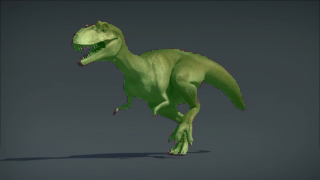
\includegraphics[scale=1.5]{new_frames/dinosaur_best/frame0}
    \caption{Segmented first frame}
    \label{fig:segmented-video}
\end{figure}



\section{Critical points}\label{sec:critical}
As previously mentioned, each video has its own characteristics and challenges, yet there are two main goals they all share.
The first is to include all the foreground pixels in the foreground image, and the second is to exclude as many background pixels as possible from the foreground image. \\
For example figure~\ref{fig:problematic-frame} shows a problematic frame from the swan video.
Notice the two marked spots, unfortunately, the tip of the swans head is excluded from the foreground image and a spot in the reflection of the swan in the water is included.
In order to fix that, achieve our goal and result in an overall better performance, there are several components we can tune in our method.
\begin{figure}
    \centering
    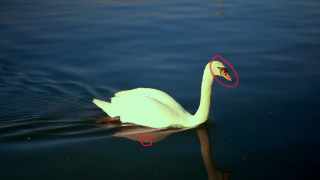
\includegraphics[scale=1.8]{images/swan/example}
    \caption{problematic frame}
    \label{fig:problematic-frame}
\end{figure}

\subsection{Including X and Y}\label{subsec:xy}
The first thing we can do is to include X and Y coordinates of each pixel in the models train data.
This should result in a better clustering process, as the pixels will be clustered not only by their color but also by their location.
The coordinates are normalized to the range [0,1] and concatenated to the color values.
If we get more accurate clusters from each model, we should get a better separation overall.
\subsection{Defining The Prior}\label{subsec:prior}
The third thing we can do is to better define the prior given to the models as input.
If we use a NIW prior, we can better customize it to fit each model.
The NIW prior is defined by the following parameters:
\begin{itemize}
    \item $\mu$ - the mean of the distribution.
    \item $\kappa$ - how much to weight the prior mean.
    \item $\nu$ - the degrees of freedom.
    \item $\phi$ - the covariance matrix.
\end{itemize}
So if we adjust these parameters according to our initial input, we can get models that better fit our data.
For each model we will use the first frame mean and covariance as \texttt{$\mu$} and \texttt{$\phi$} respectively.
$\kappa$ and $\nu$ will be set according to how much we trust our mean and covariance.
The resulting models should be better and the output gaussian mixtures should be more accurate.
\pagebreak
\subsection{Decision Rule}\label{subsec:decision}
The second thing we can do is to better define the decision rule that determines whether a pixel is foreground or background.
The simple approach is for a given pixel, calculate the probability of it belonging to each cluster and assign it to the part the cluster with the highest probability belongs to.
This approach is not wrong, but it is not optimal, as there could be situations where it would classify badly.
For instance, the probability of a pixel belonging to a single cluster in the foreground is high, but the weighted sum of probabilities of clusters in the background is much higher.
This is where a gaussian mixture would come in handy as its pdf function would classify that pixel to the background.
Yet this change did not improve the results significantly, so lets consider another case.
Consider a pixel that its probability of belonging to the foreground and background are almost equal, plus it is quite low.
We would probably be better off not classifying it in the foreground, since the foreground is usually much smaller than the background,
meaning the probability of it being in the background is probably richer as it is affected by more clusters.
This is where the threshold comes in, we can set a threshold for the probability of a pixel belonging to the foreground,
and if it is lower than that and quite close to the probability of the background, we will classify it as background.
The rule is implemented in \texttt{\_is\_pixel\_in\_object} method in \textcolor{red}{video\_object\_segmentation.py} file.
\lstinputlisting[language=Python, firstline=122, lastline=128,label={lst:pixel-in}]{../video_object_segmentation.py}
This change affects the results significantly, as now we are stricter with the pixels we classify as foreground.
So we get less false positives but also a bit less true positives that we will need to address.

\subsection{Model Adjustment}\label{subsec:model}
The last component we will address is the model adjustment.
At each iteration, after segmenting the foreground and background, we input the new images to the models and let it run a few iterations, resulting in improved gaussian mixtures.
The question is how many iterations should we run?
Intuitively, we would want to run as many iterations as possible, to let the models converge.
But the models also have a decay factor, meaning that the more iterations we run, the more the models will forget their previous inputs.
Our ground truth is the first frame, so we would want the models to remember it as much as possible, too many iterations will make the models forget it.
So we need to find a balance between the two, reducing the number of iterations at each frame to between 3 and 5 iterations, should result in better models.

\section{Results \& Conclusion}\label{sec:conclusion}
The results of our application can be viewed in the added videos, both videos (swan and dinosaur) are 5 seconds long and at 24 frames per second, so they have 120 frames each.
We also added another example of a giraffe video which is more complex and at 30 frames per second.
The segmentations are not perfect, but they are good enough to show the potential of the application. \\
In the dinosaur video, the application successfully segments the dinosaur from the background most of the video, but its legs and tail are sometimes escaping the segmentation.
This could be because the right leg starts behind the left leg in the ground-truth mask, so it begins at a disadvantage.
Also, the legs and tail are continuously moving in the depth axis, which might be a challenge for the application. \\
In the swan video, we also get good results most of the video, this is especially impressive because of the swan's reflection in the water.
Yet near the end of the video, the swan's front begins to move out of the segmentation, this could be because the decay factor is faster than the swan's movement. \\
Finally, in the giraffe video, we get a decent segmentation of the giraffe, but the flaws are more noticeable.
The part of the giraffe's that are not seen in the first frame or that are moving the most are the ones that escape the segmentation.
Considering the complexity of the video, the results are still impressive. \\
\\
In conclusion, we have successfully implemented a semi-supervised video object segmentation application that uses Or Dinari's ScStream code as a building block.
We detailed the methodology and architecture of our application and discussed the critical points that most influenced the application success.
\end{document}
